
%\newpage
\section{Измерение частоты}
\label{sec:frequency}

Начиная с версии 1.10k в меню дополнительных функций можно выбрать пункт \inquotes{Frequency} (измерение частоты). 
Стандартное измерение частоты осуществляется подсчетом количества задних фронтов входного сигнала по входу 
T0 (PD4) за одну секунду. Для получения периода счета в 1 секунду счетчик 1 используется с 
предделителем 256:1 частоты процессора.  
Для получения 1 секундного интервала за один проход можно использовать 16 разрядный счетчик ATmega 
с частотой процессора \(16~MHz\) и с предделителем.
Для запуска и остановки счетчика 0 используются регистры сравнения B и A счетчика 1. Чтобы избежать 
ошибки задержки при опросе результата сравнения сигналов событий, используются обработчики прерываний 
событий запуска и остановки счетчика 1. Времена задержек в обеих подпрограммах обслуживания прерываний 
практически равны. Для поддержания точности периода 1 секунда постоянная задержка незначительна. 
При анализе на ассемблере, разница во времени может быть скорректирована.\\

Для частот ниже \(25~kHz\) проводится стандартное измерение с последующим измерением периода времени. 
Это дополнительное измерение следует только после стандартного измерения частоты. Измерение времени 
будет сделано путем подсчета количества прерываний по входу PCINT20 (PD4) счетчиком 0.
При измерении периода импульса ширина как положительного, так и отрицательного полупериодов, 
должна быть не менее \(10~\mu s\).  
Счетчик 0 используется на максимальной тактовой частоте. Разрешение составляет  \(125~ns\) для
\(8~MHz\). При превышении подсчета периодов измерений разрешение может быть уменьшено. 
При использовании 125 периодов измерения, среднее разрешение для одного периода составит \(1~ns\). 
Для предотвращения неточности запуска и остановки счетчика 0, запуск будет
произведен по первому, а останов по последнему изменению на контакте прерывания PCINT20 по той же 
самой процедуре обслуживания прерывания. Количество периодов выбрано так, чтобы можно было измерить 
время около 10 миллионов тактов частоты процессора. При таком выборе ошибка составит 
всего \(0,1~ppm\). С тактовой частотой \(8~MHz\) время измерения составляет около 1,25 секунды. 
При определенной, таким образом, средней величине периода, частота вычисляется 
затем с более высоким разрешением.\\

Процедуру проверки проводили так: два Тестера измеряли друг друга. Первый тест: частоты генерируются 
Тестером 2 и измеряются Тестером 1. После этого Тестеры меняются местами, и измерения повторяются. 
На рисунке~\ref{fig:freq-ppm} представлены результаты обеих серий измерений. Почти постоянные 
отклонения можно объяснить небольшой разницей частот двух кварцев.

\begin{figure}[H]
\centering
\includegraphics[width=1.\textwidth]{../GNU/frequency-ppmRU.pdf}
\caption{Относительная погрешность измерения частоты}
\label{fig:freq-ppm}
\end{figure}

\subsection{Калибровка частоты по GPS- или GLONASS-приёмникам}

Подстройку частоты кварца можно осуществить установив подстроечный конденсатора (\(5-25~pF\)).
Успешно протестирована калибровка частоты кварца Тестера импульсами 1PPS с применением GPS приемника 
\textbf{ UP501} от \textbf{ Fastrax Ltd.} или с использованием GPS/GLONASS приемника \textbf{ GNS701} от \textbf{ Global 
Navigation Systems GmbH}.
Измеряемый период можно точно настроить на \(1000,000~ms\).
Только последняя цифра может отличаться на единицу.
Конечно, частота кристалла зависит от температуры. Поэтому вы не можете ожидать очень хорошую стабильность 
долгое время.

На рисунке~\ref{fig:GPS-1PPS} приведена схема подключения UM232 USB-последовательного контроллера и
приемника к компьютеру.

Конвертер UM232 автоматически поддерживает два напряжения \(5~V\) и \(3,3~V\) 
для питания схемы от USB. 

Для работы приемника подключение к компьютеру не обязательно. 
Только питание 5~V необходимо подать USB контроллеру. 

\begin{figure}[H]
  \begin{subfigure}[b]{.5\textwidth}
    \centering
    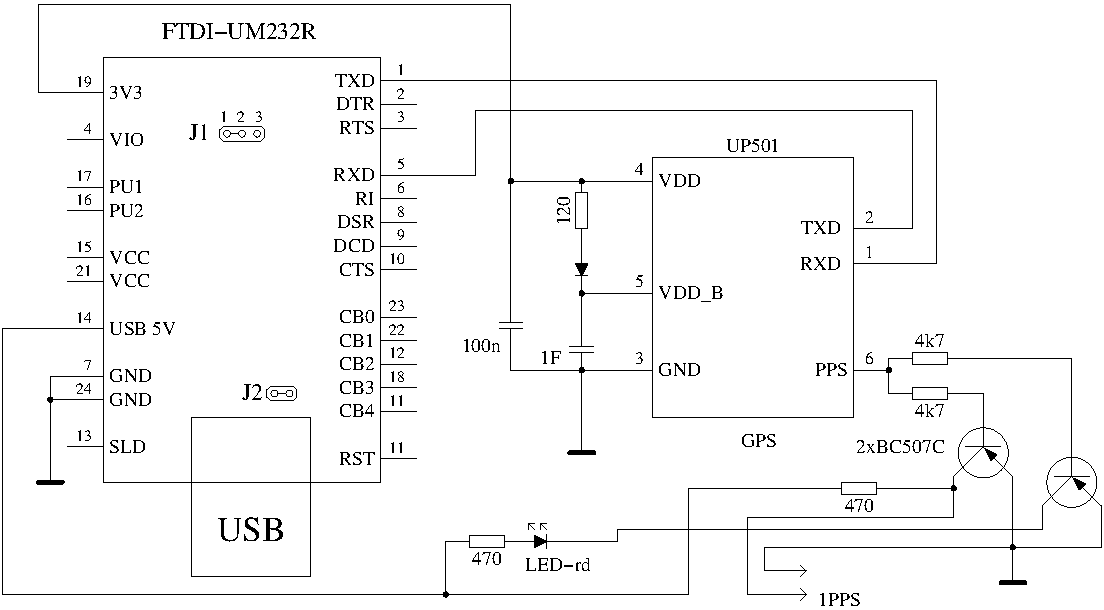
\includegraphics[width=.95\textwidth]{../FIG/GPS_UP501.pdf}
    \caption{GPS}
  \end{subfigure}
  ~
  \begin{subfigure}[b]{.5\textwidth}
    \centering
    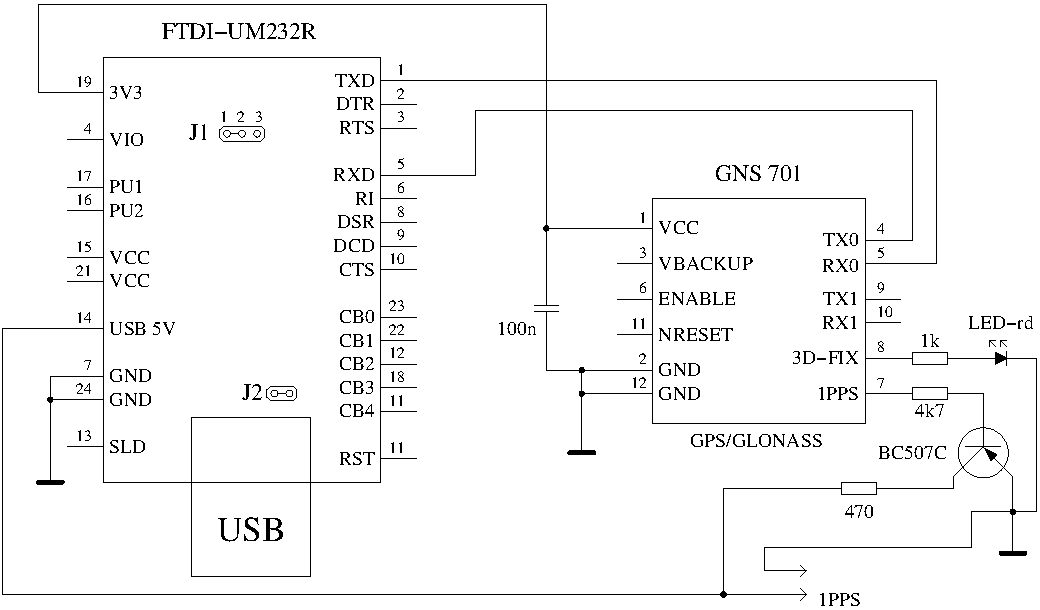
\includegraphics[width=.95\textwidth]{../FIG/GPS_GNS701.pdf}
    \caption{GPS/GLONASS}
  \end{subfigure}
  \caption{Генератор 1PPS сигнала от GPS приемника}
  \label{fig:GPS-1PPS}
\end{figure}

\subsection{Калибровка частоты с помощью тактового модуля}

Чтобы настроить частоту кристалла транзисторного тестера, вы должны сначала заменить один из
конденсаторов в обвязке кварца на триммер. Преимущество использования модулей RTC для калибровки
частоты вместо модулей GPS или GLONASS заключается в том, что Вам не нужно находиться в зоне
видимости спутника.
Вы можете настроить частоту почти в любом месте.
Я исследовал модули часов с чипом DS3231 и печатной платой с \inquotes{ZS-042}.
Обследованные модули, вероятно, производятся в Китае, и все платы оснащены чипом DS3231M.
Микросхема DS3231M использует резонатор MEMS (Micro Electro Mechanical System) вместо
чипа DS3231SN, который использует кристалл с \(32~768~Hz\).
Модифицированный резонатор MEMS также используется чипом DCP1301.
На рисунке~\ref{fig:DS3231M} показан один из используемых модулей.

\begin{figure}[H]
\centering
\includegraphics[width=.6\textwidth]{../PNG/DS3231M.jpg}
\caption{Один из протестированных DS3231 модулей}
\label{fig:DS3231M}
\end{figure}

Обе версии чипов DS3231 используют внутреннее измерение температуры для управления базовой частотой
таким образом, что дрейф частоты в широком диапазоне при изменении температуры почти полностью компенсируется.
К сожалению, предоставленный сигнал \(32~kHz\) для чипа DS3231M не может использоваться для калибровки
частоты. При измерении я получил разные частоты: \(32~641~Hz\), \(32~710~Hz\), \(32~730~Hz\) и \(32~748~Hz\) для всех 
четырех тестируемых модулей.
Все эти частоты находятся далеко от ожидаемой точной частоты \(32~768~Hz\).
Если Вы подключаете модули к Arduino UNO, Вы также можете использовать вывод 1PPS (\(1~Hz\)) с выхода SQW.
Этот выход настолько стабилен и точнен, что его можно использовать для калибровки.
Даташит DS3231M обещает для 1PPS вывода точность \(pm 5~ppm \) для полного температурного
диапазона от \(-45\celsius\) до \(+85\celsius\), а точность \(32~kHz\) на выводе
документируется только \(\pm 2.5\%\) (\(25000 ppm\)).

Лист данных чипа DS3231SN обещает точность \(pm 3,5ppm\) для полного диапазона температур
от \(-40\celsius\) до \(+85\celsius\) и точность \(\pm 2ppm\) для температуры между \(0\celsius\)
и \(+40\celsius\). В чипе DS3231SN используется внутренний тактовый кристалл с частотой \(32~768~Hz\),
частота которого стабилизируется переключаемыми конденсаторами в широком температурном диапазоне.
При известном температурном дрейфе кристалла и измерении температуры частота контролируемого кристалла почти
постоянна.
Чтобы проверить эти чипы, я заменил чипы DS3231M чипами DS3231SN для всех четырех модулей.

С откалиброванным транзисторным тестером (модель \(16~MHz\)) я измерил выходную частоту всех модулей
с одним и тем же результатом \(32,76800~kHz\). Во время измерений, очень редко, наблюдалась
разница в \(0,03~Hz\). Эта разница составляет только \(1ppm\).
Дробное количество \(1~Hz\) отображается только, если частота вычисляется для измерения периода.
Предел для измерения периода изменен с \(25~kHz\) до \(33~kHz\), чтобы сделать измерение периода
для сигнала \(32~768~Hz\) более точным.

